\chapter{Vector Calculus}

\section{Vector Fields}
A vector field in $\mathbb{R}^2$ is a function $F$ that assigns a 2D vector
$f(x,y)$ to each point $(x,y)$ in 0.

Component functions $P$ and $Q$: $F=P\ihat+Q\jhat$

A vector field on $\mathbb{R}^3$ is a function of $F$ that assigns a 3D vector
$f(x,y,z)$ to each point $(x,y,z)$ in $E$.

\subsection*{Example}
Suppose electric charge $Q$ is located at the origin. According to Coulomb's Law,
the electric force excerted at a point $(x,y,z)$ by vector $\vec{x}=\ev{x,y,z}$ is
$$F(x)=\frac{\epsilon qQ}{|\vec{x}|^3}\vec{x}$$
The force is repulsive for like charges and attractive for unlike charges. These
vector fields are known as \textbf{Force field}. Instead of considering the electric
force $F$, physicists often consider the force per unit charge:
$$E(x)=\frac{1}{q}F(x)=\frac{\epsilon Q}{|\vec{x}|^3}x$$

\subsection*{Gradient Fields}
A gradient of $\nabla f$ is defined by:
$$\nabla f(x,y)=f_x(x,y)\ihat+f_y(x,y)\jhat$$

\subsection*{Example}
Find gradient vector of $f(x,y)=x^2y-y^3$.

\textbf{Solution}
$$\nabla f(x,y)=\pdv{f}{x}\ihat +\pdv{f}{y}\jhat=2xy\ihat +(x^2-3y^2)\jhat$$
A vector field is called a \textbf{conservative vector} field if it is the gradient of some
scalar function, that is, if there exists a function $f$ such that $F=\nabla f$.
In this situation, $f$, is a \textbf{potential function} for $F$.

\section{Line Integrals}

\subsection*{Definition}
If $f$ is defined on a smooth curve $C$ given by $\left[x=x(t)\quad y=y(t)\quad
                a\leq t\leq b \right]$, then the line integral of $f$ along curve $C$ is
$$\int_C f(x,y)\:ds=\lim_{n\to\infty}\sum_{i=1}^nf(x_i^*,y_i^*)\Delta s_i$$
if this limit exists.

The following formula can also be used to evaluate a line integral:
$$\int_C f(x,y)\:ds=\int_a^b f(x(t),y(t))\sqrt{(\dv{x}{t})^2+(\dv{y}{t})^2}dt$$

\subsection*{Example}
A wire takes the shape of the semicircle $x^2+y^2=1, y \geq 0$, and is thicker
near its base than near the top. Find the center of mass of the wire if the linear
density at any point is proportional to its distance from the line $y=1$.

\textbf{Solution}
Use parametrization $x=cos\:t$, $y=sin\:t$, $0\leq t\leq\pi$, and find that $ds=dt$.
The linear density is
$$\rho(x,y)=k(1-y)$$
where $k$ is constant, and so the mass of the wire is
$$m=\int_C k(1-y)ds=\int_0^\pi k(1-sin\:t)dt=k[t+cos\:t]_0^\pi=k(\pi-2)$$
we know that the center of mass of the wire is
$$\overline{y}=\frac{1}{m}\int_C y\rho(x,y)ds=\frac{1}{k(\pi -2)}\int_C yk(1-y)ds$$
$$=\frac{1}{\pi-2}\int_0^\pi(sin\:t-sin^2\:t)dt=\frac{1}{\pi-2}\left[-cos\:t-\frac{1}{2}t+
                \frac{1}{4}sin\:2t\right]_0^\pi=\frac{4-\pi}{2(\pi-2)}$$
By symmetry we see that $\overline{x}=0$, so the center of mass is
$$\left(0, \frac{4-\pi}{2(\pi-2)}\right)\approx(0, 0.38)$$

The line integral with respect to arc length:
$$\int_C f(x,y)\:dx=\int_a^b f(x(t),t(t))\:x'(t)\:dt$$
$$\int_C f(x,y)\:dy=\int_a^b f(x(t),t(t))\:y'(t)\:dt$$
When setting up a line integral, it is often difficult to think of a parametric
representation for a curve. It's useful to remember that a vector representation
of the line segment that starts at $\textbf{r}_0$ and ends at $\textbf{r}_1$ is:
$$\textbf{r}(t)=(1-t)\textbf{r}_0+t\textbf{r}_1\qquad 0\leq t\leq 1$$
A given parametrization $x=x(t)$, $y=y(t)$, $a\leq t\leq b$, determines an
\textbf{orientation} of a curve $C$, with the positive direction corresponding to
increasing values of the parameter $t$.

If $-C$ denotes the curve of the same points as $C$ but with the opposite orientation,
then we have:
$$\int_{-C}f(x,y)\:dx=-\int_Cf(x,y)\:dx\qquad\int_{-C}f(x,y)\:dy=-\int_Cf(x,y)\:dy$$

\subsection*{Line Integrals in Space}
Suppose that $C$ is now a smooth curve. We define the line integral along $C$
(with respect to arc length) in a manner similar to that for plane curves:
$$\int_Cf(x,y,z)\:ds=\int_a^bf(x(t),y(t),z(t))\sqrt{\left(\dv{x}{t}\right)^2+
                \left(\dv{y}{t}\right)^2+\left(\dv{z}{t}\right)^2}dt$$
The integral can also be written as:
$$\int_a^bf(\textbf{r}(t))|\textbf{r}'(t)|\:dt$$

\subsection*{Example}
Evaluate $\int_Cysin\:z\:ds$, where $C$ is the circular helix given by $x=cos\:t$,
$y=sin\:t$, $z=t$, $0\leq t\leq 2\pi$.

\subsection*{Solution}
\begin{align*}
        \int_Cysin\:z\:ds & =\int_0^{2\pi}(sin\:t)sin\:t\sqrt{\left(\dv{x}{t}\right)^2+\left(\dv{y}{t}\right)^2+\left(\dv{z}{t}\right)^2}dt \\
                          & =\int_0^{2\pi}sin^2t\sqrt{sin^2t+cos^2t+1}\:dt=\sqrt{2}\int_0^{2\pi}\frac{1}{2}(1-cos\:2t)\:dt                  \\
                          & =\frac{\sqrt{2}}{2}\left[t-\frac{1}{2}sin\:2t\right]_0^{2\pi}=\sqrt{2}\pi
\end{align*}

\subsection*{Line Integrals of Vector Fields}
$$W=\int_C\textbf{F}(x,y,z)\cdot\textbf{T}(x,y,z)\:ds=\int_C\textbf{F}\cdot\textbf{T}\:ds$$
Work is the line integral with respect to arc length of the tangetial component
for the force.

\subsection*{Definition}
Let $F$ be a continous vector field defined on a smooth curve $C$ given by a vector
function $\textbf{r}(t)$, $a\leq t\leq b$. Then the \textbf{line integral of $F$
        along $C$} is
$$\int_C\textbf{F}\cdot d\textbf{r}=\int_a^b\mathbf{F(r}(t))\cdot\textbf{r}'(t)\:dt=\int_C\mathbf{F\cdot T}\:ds$$

\subsection*{Example}
Find the work done by the force field $\textbf{F}(x,y)=x^2\ihat-xy\jhat$ in moving a
particle along the quarter-circle $\textbf{r}(t)=cos\:t\ihat+sin\:t\jhat$,
$0\leq t\leq\pi/2$.

\textbf{Solution} \\
Since $x=cos\:t$ and $y=sin\:t$, we have
$$\mathbf{F(r}(t))=cos^2t\ihat-cos\:tsin\:t\jhat$$
$$\textbf{r}'(t)=-sin\:t\ihat+cos\:t\jhat$$
Therefore the work done is:
$$\int_C\textbf{F}\cdot d\textbf{r}=\int_0^{\pi/2}\mathbf{F(r}(t))\cdot\textbf{r}'(t)\:dt=
        \int_0^{\pi/2}(-2cos^2t\:sin\:t)\:dt=\left[2\frac{cos^3t}{3}\right]_0^{\pi/2}=-\frac{2}{3}$$

\section{The Fundamental Theorem for Line Integrals}

The Fundamental Theorem of Calculus is:
$$\int_a^b F'(x)\:dx=F(B)-F(a)$$

\subsection*{Theorem}
Let $C$ be a smooth curve given by the vector function $r(t)$, $a\leq t\leq b$.
Let $f$ be a differentiable functino of two or three variables whose gradient vector
$\nabla f$ is continous.
$$\int_C \nabla f\cdot dr=f(r(b))-f(r(a))$$

\subsection*{Proof}
Using the line integral, we have
\begin{align*}
        \int_C \nabla f\cdot dr & =\int_a^b\nabla f(r(t))\cdot r'(t)\:dt                                                   \\
                                & =\int_a^b\left(\pdv{f}{x}\pdv{x}{t}+\pdv{f}{y}\pdv{y}{t}+\pdv{f}{z}\pdv{z}{t}\right)\:dt \\
                                & =\int_a^b \frac{d}{dt} f(r(t))\:dt                                                       \\
                                & =f(r(b))-f(r(a))
\end{align*}

\subsection*{Independence of Path}
If $F$ is a continous vector field with domain $D$, we say that the line integral
$\int_c F\cdot dr$ is independent of path if $\int_{C_1}F\cdot dr=\int_{C_2}F\cdot dr$
for any two paths $C_1$ and $C_2$ in $D$ that have the same initial and terminal paths.

A curve is called closed if $r(b)=r(a)$.

\subsection*{Theorem}
$\int_C F\cdot dr$ is independent of path in $D$ if and only if $\int_C F\cdot dr=0$
for every closed path $C$ in $D$.

\subsection*{Proof}
$$\int_C F\cdot dr=\int_{C_1} F\cdot dr+\int_{C_2} F\cdot dr=\int_{C_1} F\cdot dr-\int_{-C_2} F\cdot dr=0$$
Conversely, if that is true, do the same thing backwards to prove it is closed.

$D$ is open $\to$ for every point $P$ in $D$ there is no disk with center $P$ that
lies entirely on $D$.

$D$ is connected $\to$ any two points in $D$ can be joined by a path in $D$.

\subsection*{Theorem}
$F$ is a vector field that is continous in an open connected region in $D$. If
$\int_C F\cdot dr$ is independent of path in $D$, then $F$ is a conservative vector
field in $D$ where a function $f$ that $\nabla f=F$ exist.

\subsection*{Theorem}
If $F(x,y)+P(x,y)\ihat+Q(x,y)\jhat$ is a conservative vector field, where $P$ and $Q$
have continous first-order partial derivatives on a domain $D$, then through $D$ we have
$$\pdv{P}{y}=\pdv{Q}{x}$$

\subsection*{Theorem}
Let $F+P\ihat + Q\jhat$ be a vector field on an open simply-connected region $D$.
Supposed that $P$ and $Q$ have continous first-order derivatives and
$\pdv{P}{y}=\pdv{Q}{x}$ throughout $D$. Then $F$ is conservative.

\subsection*{Example}
Determine whether or not $F(x,y)=(x,y)\ihat+(x,z)\jhat$ is conservative.

\subsection*{Solution}
Let $P(x,y)=x-y$ and $Q(x,y)=x-z$
$$\text{then} \qquad \pdv{P}{y}=-1 \qquad \pdv{Q}{x}=1$$
since $\pdv{P}{y}\neq\pdv{Q}{x}$, $F$ is not conservative.

\section{Green's Theorem}
Green's Theorem gives the relationship between a line integral around a simpled
curve $C$ and a double integral over the plane region $D$ bounded by $C$.

\subsection*{Green's Theorem}
Let $C$ be a positively oriented, piecewise-smooth, simple closed curve in the plane
and let $D$ be the region bounded by $C$. If $P$ and $Q$ have continous partial derivatives
on an open region that contains $D$, then
$$\int\_C P\:dx+Q\:dy=\iint\limits_D\left(\pdv{Q}{x}-\pdv{P}{y}\right)\:dA$$

\subsection*{Proof}
For the case in with $D$ is a simple region
\begin{enumerate}
        \item[] $D=\{(x,y)\:|\:a\leq x\leq b,\:g_1(x)\leq y\leq g_2(x)\}$
        \item[] $\iint\limits_D \pdv{P}{y}\:dA=\int_a^b\int_{g_1(x)}^{g_2(x)}\pdv{P}{y}(x,y)\:dy\:dx=
                      \int_a^b \left[P(x,g_2(x))-P(x,g_1(x))\right]\:dx$
        \item[] $\int_{C_1} P(x,y)\:dx=\int_a^b P(x,g(1(x)))\:dx$
        \item[] $\int_{C_3} P(x,y)\:dx=-\int_{-C_3} P(x,y)\:dx=-\int_a^b P(x,g_2(x))\:dx$
        \item[] $\int_{C_2} P(x,y)\:dx=0=\int_{C_4} P(x,y)\:dx$
        \item[] $\int_C P(x,y)\:dx=\int_{C_1} P(x,y)\:dx+\int_{C_2} P(x,y)\:dx+\int_{C_3} P(x,y)\:dx$
        \item[] $+\int_{C_4} P(x,y)\:dx$
        \item[] $\int_a^b P(x,g_1(x))\:dx-\int_a^b P(x,g_2(x))\:dx$
        \item[] $\int_C P(x,y)\:dx=-\iint\limits_D \pdv{P}{y}\:dA$
\end{enumerate}

\subsection*{Example}
Evaluate $\oint_C (3y-c^{\sin{x}})\:dx+(7x+\sqrt{y^4+1})\:dy$, where $C$ is the circle
$x^2+y^2=9$.

\subsection*{Solution}
The region $D$ bounded by $C$ is the disk $x^2+y^2\leq 9$ so let's change to polar
coordinates after applying Green's Theorem:
$$\oint_C (3y-c^{\sin{x}})\:dx+(7x+\sqrt{y^4+1})\:dy$$
$$=\iint\limits_D \left[\frac{\partial}{\partial x}(7x+\sqrt{y^4+1})-\frac{\partial}{\partial y}
                (3y-e^{\sin{x}})\right]\:dA$$
$$=\int_0^{2\pi}\int_0^3 (7-3)\:r\:dr\:d\theta=4\int_0^{2\pi}d\theta\int_0^3r\:dr=36\pi$$

The Green's Theorem gives the following formulas for the area of $D$:
$$A=\oint_C x\:dy=-\oint_C y\:dx=\frac{1}{2}\oint_C x\:dy-y\:dx$$

\subsection*{Example}
Find the area enclosed by the ellipse $\cfrac{x^2}{a^2}+\cfrac{y^2}{b^2}=1$.

\subsection*{Solution}
The ellipse has parametric equations $x=a\cos{t}$ and $y=b\sin{t}$, where $0\leq t\leq 2\pi$.
Using the formula for area from above, we have
$$A=\frac{1}{2}\int_C x\:dy-y\:dx$$
$$\frac{1}{2}\int_0^{2\pi}(a\cos{t})(b\cos{t})\:dt-(b\sin{t})(-a\sin{t})\:dt$$
$$\frac{ab}{2}\int_0^{2\pi}dt=\pi ab$$

\section{Curl and Divergence}

\subsection*{Curl}
If $F+P\ihat+Q\jhat+R\khat$ is a vector field on $\mathbb{R}^3$ and the partial
derivatives of $P$, $Q$, and $R$ all exist, then the \textbf{curl} of $F$ is the
vector field on $\mathbb{R}^3$ defined by
$$\text{curl F}=\left(\pdv{R}{y}-\pdv{Q}{z}\right)\ihat+\left(\pdv{P}{z}-\pdv{R}{x}\right)\jhat+
        \left(\pdv{Q}{x}-\pdv{P}{y}\right)\khat$$
$$\text{or} \qquad \text{curl F}=\nabla \times F$$

\subsection*{Example}
$F(x,y,z)=xz\ihat+xyz\jhat-y^2\khat$, find curl F.

\subsection*{Solution}
\begin{align*}
        \text{curl F} & =\nabla \times F=\begin{vmatrix}
                \ihat                        & \jhat                        & \khat                        \\
                \dfrac{\partial}{\partial x} & \dfrac{\partial}{\partial y} & \dfrac{\partial}{\partial z} \\
                xz                           & xyz                          & -y^2
        \end{vmatrix}                                             \\
                      & =\left[\frac{\partial}{\partial y}(-y^2)-\frac{\partial}{\partial z}(xyz)\right]\ihat-
        \left[\frac{\partial}{\partial x}(-y^2)-\frac{\partial}{\partial z}(xz)\right]                         \\
                      & +\left[\frac{\partial}{\partial x}(xyz)-\frac{\partial}{\partial y}(xz)\right]         \\
                      & =(-2y-xy)\ihat-(0-x)\jhat+(yz-0)\khat                                                  \\
                      & =-y(2+x)\ihat+x\jhat+yz\khat
\end{align*}

\subsection*{Theorem}
If $F=P\ihat+Q\jhat+R\khat$ is a vector field on $\mathbb{R}^3$ and $P$, $Q$, and $R$
have continous second-order partial derivatives, then
$$\text{div curl F}=0$$

\subsection*{Proof}
Using the definitions of divergence and curl, we have
$$\text{div curl F}=\nabla\cdot(\nabla\times \textbf{F})$$
$$=\frac{\partial}{\partial x}\left(\pdv{R}{y}-\pdv{Q}{z}\right)+
        \frac{\partial}{\partial y}\left(\pdv{P}{z}-\pdv{R}{x}\right)+
        \frac{\partial}{\partial z}\left(\pdv{Q}{x}-\pdv{P}{y}\right)$$
$$=\pdv{R}{x}{y}-\pdv{Q}{x}{z}+\pdv{P}{y}{z}-\pdv{R}{y}{x}+\pdv{Q}{z}{x}-\pdv{P}{z}{y}$$
$$=0$$

\subsection*{Vector Forms of Green's Theorem}
$F=P\ihat+Q\jhat$, its line integral is:
$$\oint_C F\cdot dr=\oint_C P\:dx + Q\:dy$$
and its curl is:
$$\text{curl F}=\begin{vmatrix}
                \ihat     & \jhat     & \khat     \\
                \pdv{}{x} & \pdv{}{y} & \pdv{}{z} \\
                P(x,y)    & Q(x,y)    & 0
        \end{vmatrix}=
        \left(\pdv{Q}{x}-\pdv{P}{y}\right)\khat$$
Therefore
$$\text{curl F}\cdot \khat = \left(\pdv{Q}{x}-\pdv{P}{y}\right)\khat\cdot\khat=\pdv{Q}{x}-\pdv{P}{y}$$
and we can now rewrite the equation in Green’s Theorem in the vector form
$$\oint_C F\cdot dr=\iint\limits_D (\text{curl F})\cdot\khat\:dA$$

A similar function involving the \textbf{normal} component of $F$:
$$\oint_C F\cdot n\:ds=\iint\limits_D \text{div F}(x,y)\:dA$$

\section{Parametric Surfaces and Their Areas}

\subsection*{Parametric Surfaces}
The set of all points $(x,y,z)$ in $\mathbb{R}^3$ such that
$$x=x(u,v) \qquad y=y(u,v) \qquad z=z(u,v)$$
and $(u,v)$ varies through $D$, is called a \textbf{parametric surface} $S$.

\subsection*{Example}
Identify and sketch the surface with vector equation
$$r(u,v)=2\cos{u}\ihat + v\jhat + 2\sin{u}\khat$$

\subsection*{Solution}
The parametric equations for this surface are
$$x=2\cos{u}\qquad y=v \qquad z=2\sin{u}$$
So for any point $(x,y,z)$ on the surface, we have
$$x^2+z^2=4\cos^2{u}+4\sin^2{u}=4$$
Since $y=v$ and no restriction is placed on $v$, the surface  is a circular cylinder with radius 2 whose axis is the $y$-axis.
\begin{center}
        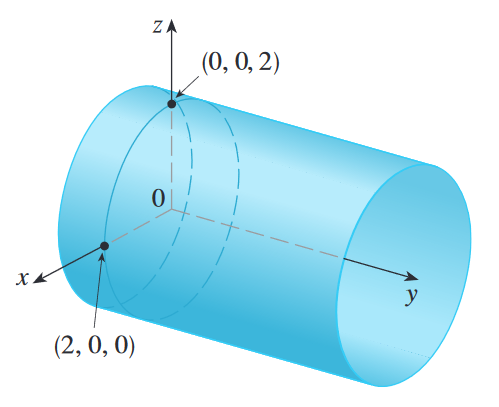
\includegraphics[scale=0.5]{example17-6-1.png}
\end{center}

\subsection*{Tangent Planes}
The tangent vector to $C_1$ at $P_0$ is obtained by taking the partial derivative
of $r$ with respect to $v$:
$$r_v=\pdv{x}{v}(u_0,v_0)\ihat+\pdv{y}{v}(u_0,v_0)\jhat+\pdv{z}{v}(u_0,v_0)\khat$$
Same thing fo $r_u$ but $\partial v$ changes to $\partial u$.

If $r_u\times r_v$ is not 0, the surface $S$ is called smooth (has no corners).
For a smooth surface, the \textbf{tangent plane} is the plane that contains $r_u$ and
$r_v$, and the vector $r_u\times r_v$ is a normal vector to the tangent plane.

\subsection*{Example}
Find the tangent plane to the surface with parametric equations $x=u^2$, $y=v^2$,
$z=u+2v$ at the point (1, 1, 3).

\subsection*{Solution}
We first compute the tangent vectors:
$$r_u=\pdv{x}{u}\ihat+\pdv{y}{u}\jhat+\pdv{z}{u}\khat=2u\ihat+\khat$$
$$r_v=\pdv{x}{v}\ihat+\pdv{y}{v}\jhat+\pdv{z}{v}\khat=2v\jhat+\khat$$
Thus a normal vector to the tangent plane is
$$r_u\times r_v=\begin{vmatrix}
                \ihat & \jhat & \khat \\
                2u    & 0     & 1     \\
                0     & 2v    & 2
        \end{vmatrix}=-2v\ihat-4u\jhat+4uv\khat$$
The point (1, 1, 3) corresponds to the parameter values $u=1$ and $v=1$, so the normal vector there is
$$-2\ihat-4\jhat+4\khat$$
Therefore an equation of the tangent plane at (1, 1, 3) is
$$-2(x-1)-4(y-1)+4(z-3)=0$$
$$\text{or} \qquad x+2y-2z+3=0$$

\subsection*{Surface Area}
$$A(S)=\iint\limits_D \sqrt{1+\left(\pdv{z}{x}\right)^2+\left(\pdv{z}{y}\right)^2}\:dA$$

\subsection*{Example}
Find the area of the part of the paraboloid $z=x^2+y^2$ that lies under the plane $z=9$.

\subsection*{Solution}
The plane intersects the paraboloid in the circle $x^2+y^2=9$, $z=9$. Therefore the
given surface lies above the disk $D$ with center the origin and radius 3.
\begin{align*}
        A & =\iint\limits_D \sqrt{1+\left(\pdv{z}{x}\right)^2+\left(\pdv{z}{y}\right)^2}\:dA \\
          & =\iint\limits_D\sqrt{1+(2x)^2+(2y)^2}\:dA                                        \\
          & =\iint\limits_D\sqrt{1+4(x^2+y^2)}\:dA
\end{align*}
Converting to polar coordinates, we obtain
\begin{align*}
        A & =\int_0^{2\pi}\int_0^3 \sqrt{1+4r^2}\:r\:dr\:d\theta=\int_0^{2\pi}d\theta\int_0^3r\sqrt{1+4r^2}\:dr  \\
          & =\left[2\pi\left(\frac{1}{8}\right)\frac{2}{3}(1+4r^2)^{3/2}\right]_0^3=\frac{\pi}{6}(37\sqrt{37}-1)
\end{align*}

\section{Surface Integrals}
Surface integral of $f$ over the surface $S$:
$$\iint\limits_S f(x,y,z)\:dS=\iint\limits_D f(x,y,g(x,y))\sqrt{\left(\pdv{z}{x}\right)^2+
                \left(\pdv{z}{y}\right)^2+1}\:dA$$

\subsection*{Example}
Evaluate $\iint\limits_S y\:dS$, where $S$ is the surface $z=x+y^2$, $0\leq x\leq 1$,
$0\leq y\leq 2$.

\subsection*{Solution}
Since
$$\pdv{z}{x}=1 \qquad \text{and} \qquad \pdv{z}{y}=2y$$
\begin{align*}
        \iint\limits_S y\:dS & =\iint\limits_D y\sqrt{1+\left(\pdv{z}{x}\right)^2+\left(\pdv{z}{y}\right)^2}\:dA                \\
                             & =\int_0^1\int_0^2 y\sqrt{1+1+4y^2}\:dy\:dx                                                       \\
                             & =\int_0^1 dx\sqrt{2}\int_0^2 y\sqrt{1+2y^2}\: dy                                                 \\
                             & =\left[\sqrt{2}\left(\frac{1}{4}\right)\frac{2}{3}(1+2y^2)^{3/2}\right]_0^2=\frac{13\sqrt{2}}{3}
\end{align*}

\subsection*{Surface Integrals of Vector Fields}
The mass of a fluid crossing $S_{ij}$ in the direction of the normal $n$ per unit
time by the quantity
$$(pv\cdot n)A(S_{ij})$$
where $p$, $v$, and $n$ are evaluated at some point on $S_{ij}$.
$$\iint\limits_S pv\cdot n\:dS=\iint\limits_S p(x,y,z)v(x,y,z)\cdot n(x,y,z)\:dS$$
is the rate of flow through $S$.

If we write $F=pv$, then $F$ is also a vector field on $\mathbb{R}^3$ and the integral above becomes
$$\iint\limits_S F\cdot n\:dS$$

\subsection*{Definition}
If  $F$ is a continuous vector field defined on an oriented surface $S$ with unit normal
vector $n$, then the \textbf{surface integral of $F$ over $S$} is
$$\iint\limits_S F\cdot dS=\iint\limits_S F\cdot n\:dS$$
This integral is also called the \textbf{flux} of $F$ across F.

It can also be written as:
$$\iint\limits_S F\cdot dS=\iint\limits_D\left(-P\pdv{g}{x}-Q\pdv{g}{y}+R\right)\:dA$$

\subsection*{Example}
Evaluate $\iint_S F\cdot dS$, where $F(x,y,z)=y\ihat+x\jhat+z\khat$ and $S$ is the
boundary of the solid region $E$ enclosed by the paraboloid $z=1-x^2-y^2$ and the plane $z=0$.

\subsection*{Solution}
$$P(x,y,z)=y \qquad Q(x,y,z)=x \qquad R(x,y,z)=z=1-x^2-y^2$$
$$\pdv{g}{x}=-2x \qquad \text{and} \qquad \pdv{g}{y}=-2y$$
\begin{align*}
        \iint\limits_{S_1} F\cdot dS & =\iint\limits_D\left(-P\pdv{g}{x}-Q\pdv{g}{y}+R\right)\:dA                                      \\
                                     & =\iint\limits_D[-y(-2x)-x(-2y)+1-x^2-y^2]\:dA                                                   \\
                                     & =\iint\limits_D(1+4xy-x^2-y^2)\:dA                                                              \\
                                     & =\int_0^{2\pi}\int_0^1(1+4r^2\cos{\theta}\sin{\theta}-r^2)\:r\:dr\:d\theta                      \\
                                     & =\int_0^{2\pi}\int_0^1(r-r^3+4r^3\cos{\theta}\sin{\theta})\:dr\:d\theta                         \\
                                     & =\int_0^{2\pi}(\frac{1}{4}+\cos{\theta}\sin{\theta})\:d\theta=\frac{1}{4}(2\pi)+0=\frac{\pi}{2}
\end{align*}

The disk $S_2$ is oriented downward, so its unit normal vector is $n=-\khat$ and we have
$$\iint\limits_{S_2} F\cdot dS=\iint\limits_{S_2} F\cdot(-\khat)\:dS=\iint\limits_D
        (-z)\:dA=\iint\limits_D 0\:dA=0$$
$$\iint\limits_S F\cdot dS=\iint\limits_{S_1}F\cdot dS+\iint\limits_{S_2}F\cdot dS=
        \frac{\pi}{2}+0=\frac{\pi}{2}$$

\section{Stokes Theorem}

\subsection*{Stokes Theorem}
Let  $S$ be an oriented piecewise-smooth surface that is bounded by a simple, closed,
piecewise-smooth boundary curve $C$ with positive orientation. Let $F$ be a vector
field whose components have continuous partial derivatives on an open region in
$\mathbb{R}^3$ that contains $S$. Then
$$\int_C F\cdot dr=\iint\limits_S \text{curl F}\cdot dS$$

\subsection*{Proof}
\begin{align*}
        \oint F\cdot dr & =\iint(\nabla\times\bar{F})\cdot dA=\int(F_xdx+F_ydy+F_zdz)                                                  \\
                        & =\int(\int dF_xdx)+\int(\int dF_ydy)+\int(\int dF_zdz)                                                       \\
                        & =\int(\int \pdv{F_x}{y}dy+\pdv{F_x}{z}dz)dx+\int(\pdv{F_y}{x}dx+\pdv{F_y}{z}dz)dy                            \\
                        & +\int(\pdv{F_z}{x}dx+\pdv{F_z}{y}dy)dz)                                                                      \\
                        & \text{order of integration matters: }dx\times dy=-dy\times dx                                                \\
                        & =\int(\int-\pdv{F_x}{y}dxdy+\pdv{F_x}{z}dzdx)+(\int\pdv{F_y}{x}dxdy-\pdv{F_y}{z}dydz)                        \\
                        & +\int(-\pdv{F_z}{x}dzdx+\pdv{F_z}{y}dydz)                                                                    \\
                        & =\int(\pdv{F_z}{y}-\pdv{F_y}{z})dydz+\int(\pdv{F_y}{z}-\pdv{F_z}{x})dzdx+\int(\pdv{F_y}{x}-\pdv{F_x}{y})dxdy \\
                        & =\int(\int \nabla\times F)_x dA_x + (\int \nabla\times F)_y dA_y + (\int \nabla\times F)_z dA_z              \\
                        & =\iint(\nabla\times\bar{F}\cdot d\bar{A})
\end{align*}

\subsection*{Example}
Use Stokes’ Theorem to compute the integral $\iint_S \text{curl F}\cdot dS$, where
$F(x,y,z)=xz\ihat+yz\jhat+xy\khat$ and $S$ is the part of the sphere $x^2+y^2+z^2=4$
that lies inside the cylinder $x^2+y^2=1$ and above the $xy$-plane.

\subsection*{Solution}
To find the boundary curve $C$ we solve the equations $x^2+y^2+z^2=4$ and $x^2+y^2=1$.
Subtracting, we get $z^2=3$ and so $z=\sqrt{3}$. Thus $C$ is the circle given by the
equations $x^2+y^2=1$, $z=\sqrt{3}$. A vector equation of $C$ is
$$r(t)=\cos{t}\ihat+\sin{t}\jhat+\sqrt{3}\khat \qquad 0\leq t\leq 2\pi$$
$$r'(t)=-\sin{t}\ihat+cos{t}\jhat$$
$$F(r(t))=\sqrt{3}\cos{t}\ihat+\sqrt{3}\sin{t}\jhat+\cos{t}\sin{t}\khat$$
Therefore, by Stokes' Theorem
$$\iint\limits_S \text{curl F}\cdot dS=\int_C F\cdot dr=\int_0^{2\pi} F(r(t))\cdot r'(t)\:dt$$
$$=\int_0^{2\pi}(-\sqrt{3}\cos{t}\sin{t}+\sqrt{3}\sin{t}\cos{t})\:dt$$
$$\sqrt{3}\int_0^{2\pi}0\:dt=0$$

\section{Divergence Theorem}

\subsection*{The Divergence Theorem}
Let $E$ be a simple solid region and let $S$ be the boundary surface of $E$,
given with positive (outward) orientation. Let $F$ be a vec­tor field whose
component functions have continuous partial derivatives on an open region that
contains $E$. Then
$$\iint\limits_S F\cdot dS=\iiint\limits_E \text{div F}\:dV$$

\subsection*{Proof}
\begin{align*}
        \oiint \bar{F}\cdot d\bar{S} & =\iint(F_xdA_x+F_ydA_y+F_zdA_z)                                    \\
                                     & =\iint F_xdydz + F_ydzdx + F_zdxdy                                 \\
                                     & =\iiint (\pdv{F_x}{x}dxdydz+\pdv{F_y}{y}dydzdx+\pdv{F_z}{z}dzdxdy) \\
                                     & =\iiint \nabla \bar{F}\:dV
\end{align*}

\subsection*{Example}
Find the flux of the vector field $F(x,y,z)=z\ihat+y\jhat+x\khat$ over the unit
sphere $x^2+y^2+z^2=1$.

\subsection*{Solution}
First we compute the divergence of $F$:
$$\text{div F}=\pdv{}{x}(z)+\pdv{}{y}(y)+\pdv{}{z}(x)=1$$
The unit sphere $S$ is the boundary of the unit ball $B$ given by $x^2+y^2+z^2\leq 1$.
Thus the Divergence Theorem gives the flux as
$$\iint\limits_S F\cdot dS = \iiint\limits_B 1\:dV=V(B)=\frac{4}{3}\pi(1)^3=\frac{4\pi}{3}$$